\documentclass{article}
\usepackage{lipsum}
\usepackage{fancyhdr}
\usepackage{graphicx}
\usepackage[all]{xy}
\usepackage{amsmath, amsthm, latexsym, amssymb, graphicx,color,cite,mathabx,enumerate,mathrsfs}
\usepackage[left=2.0 cm,right=2.0cm,top=3cm,bottom=3cm]{geometry}
\pagenumbering{arabic}
\pagestyle{fancy}
\rhead{HUAN Q. BUI}
\usepackage{dsfont}
\newtheorem{theorem}{Theorem}
\newtheorem{fact}{Fact}
\newtheorem{lemma}{Lemma}
\newtheorem{definition}{Definition}
\newtheorem{corollary}{Corollary}
\newtheorem{proposition}{Proposition}
\newtheorem{remark}{Remark}
\newtheorem{notation}{Notation}
\newtheorem{example}{Example}
\newtheorem{non-example}{Non-example}
\renewcommand{\Re}{\operatorname{Re}}%%redefined Re and Im
\renewcommand{\Im}{\operatorname{Im}}
\newcommand{\tr}{\operatorname{tr}}
\renewcommand{\det}{\operatorname{det}}
\newcommand{\cadlag}{\textit{c\'{a}dlag} }
\newcommand{\E}{\mathbb{E}}%notation for expectation
\newcommand{\unit}[1]{\overline{\underline{#1}}}%notation for the unit contraction function

\usepackage{amsmath}
%\usepackage{svgcolor}
\usepackage[svgnames]{xcolor}
\usepackage[framemethod=tikz]{mdframed}


\newcommand{\p}{\partial}
\newcommand{\R}{\mathbb{R}}
\newcommand{\C}{\mathbb{C}}
\newcommand{\lag}{\mathcal{L}}
\newcommand{\I}{\mathcal{I}}
\newcommand{\K}{\mathcal{K}}
\newcommand{\F}{\mathcal{F}}
\newcommand{\w}{\omega}
\newcommand{\lam}{\lambda}
\newcommand{\al}{\alpha}
\newcommand{\be}{\beta}
\newcommand{\x}{\xi}

\newcommand{\f}[2]{\frac{#1}{#2}}

\newcommand{\ift}{\infty}

\newcommand{\lp}{\left(}
\newcommand{\rp}{\right)}

\newcommand{\lb}{\left[}
\newcommand{\rb}{\right]}

\newcommand{\lc}{\left\{}
\newcommand{\rc}{\right\}}


\title{Calculus of Variations\\in\\Partial Differential Equations}
\author{Huan Q. Bui}
\date{May 18, 2019}
\begin{document}
\pagenumbering{roman}
\maketitle
\begin{center}
\includegraphics[scale=0.55,angle=270]{intro.eps}\\
\end{center}



\newpage
\tableofcontents
\newpage
\pagenumbering{arabic}

\section{Introduction}

One of the many things I love about studying both physics and mathematics is seeing how ideas in one field can connect to ideas in the other. 



\section{Calculus of Variations}

From an applied viewpoint, calculus of variations poses a fascinating indirect approach to solving optimization problems: considering small deviations from a solution (variations) and finding solutions based on what makes non-solutions are sub-optimal. In a way, the idea of calculus of variations is much like the scientific process where the necessary conditions for the truth - a solution to a problem, or a theory of a natural phenomenon - is often obtained by trial and error. It is thus not surprising that calculus of variation gives a \textit{natural} method for finding physical laws. Calculus of variations appears in almost all corners of physics, often under the name of the Principle of Least Action. Lagrangian's formalism of classical mechanics gives solutions so natural and elegant that it has supersedes Newtonian mechanics. The principle of least action is also one of the fundamental ideas of classical and quantum field theory. Once-postulated Einstein's field equations and Schr\"{o}dinger's equation turned out to be derivable from calculus of variations.   

\subsection{Euler-Lagrange's Equation}

Suppose we want to find the shortest arc joining two points on a plane. We are certain that the arc is a straight line. But how is a straight line joining two points is the shortest arc? The idea of calculus of variations is to consider a solution $\bar{y}(x)$ that minimizes the distance $S$ between the two points, say $A(x_1,y_1)$ and $B(x_2,y_2)$, and some deviation $\eta(x)$ from this correct curve $\bar{y}(x)$. Thus any deviation from the correct path associated with $\eta(x)$ can be written as
\begin{align}
y(x) = \bar{y}(x) + \epsilon \eta(x)
\end{align}
where $\eta$ is a constant parameter controlling for the magnitude of the deviation $\eta(x)$. Since we want the end points of any general path to be the same as the correct path, it is required that $\eta(x_1) = \eta(x_2) = 0$.\\

The distance $S(\epsilon)$ between $A$ and $B$ for any given $\eta(x)$ can be found by a little bit of calculus:
\begin{align}
S(\epsilon) = \int^{x_2}_{x_1}\sqrt{1 + \left(\frac{dy}{dx}\right)^2}\,dx.
\end{align}

Before solving this problem, let us think about a more general case. Let the integrand be $f = f(y',y,x) = f(\bar{y}'+\epsilon\eta',y+\epsilon\eta,x)$, where $x$ is the ``independent'' variable and $f$ is admissible. Since we require that $S$ is minimized, $dS(\epsilon)/d\epsilon = 0$. Thus it is necessary that
\begin{align}\label{exp}
0 &= \f{dS}{d\epsilon} \nonumber\\ 
&= \f{d}{d\epsilon}\int^{x_2}_{x_1}f(\bar{y}'+\epsilon\eta',y+\epsilon\eta,x)\,dx \nonumber\\
&= \int^{x_2}_{x_1}\f{d}{d\epsilon}f(\bar{y}'+\epsilon\eta',y+\epsilon\eta,x)\,dx \nonumber\\
&= \int^{x_2}_{x_1}\f{d}{d\epsilon}f(\bar{y}'+\epsilon\eta',y+\epsilon\eta,x)\,dx \nonumber\\
&= \int^{x_2}_{x_1}\eta'\f{\p f}{\p y'} + \eta\f{\p f}{\p y}\,dx 
\end{align}

Consider the first term in the integrand. Integrating by parts gives.
\begin{align}\label{bounds}
\int^{x_2}_{x_1}\eta'\f{\p f}{\p y'} \,dx
&= \eta\f{\p f}{\p y'}\bigg\vert_{x_1}^{x_2} -  \int^{x_2}_{x_1}  \f{d}{dx}\f{\p f}{\p y} \,dx \nonumber\\
&= -  \int^{x_2}_{x_1}  \f{d}{dx}\f{\p f}{\p y} \,dx,
\end{align} 
where the boundary term vanishes due to the constraint $\eta(x_1) = \eta(x_2) = 0$. From \eqref{exp} and \eqref{bounds}, we have
\begin{align}
0 = \int^{x_2}_{x_1} \eta\lp \f{\p f}{\p y} - \f{d}{dx}\f{\p f}{\p y'}  \rp\,dx. 
\end{align}

Now, because we require that $\bar{y}(x)$ minimizes $S$ and that this holds for any deviation $\eta(x)$ from $\bar{y}(x)$, we obtain the \textbf{Euler-Lagrange equation}. 
\begin{align}
\boxed{\f{\p f}{\p y} - \f{d}{dx}\f{\p f}{\p y'} = 0}
\end{align}

Back to our original problem with finding the shortest arc joining two points on a plane. We have that
\begin{align}
f(y',y,x) = \sqrt{1 + \lp\f{dy}{dx}\rp^2}.
\end{align}
Thus,
\begin{align}
\f{\p f}{\p y} &= 0\\
\f{\p f}{\p y'} &= \f{1}{2}\f{2y'}{\sqrt{1 + y'^2}} = \f{y'}{\sqrt{1 + y'^2}}.
\end{align}
By the Euler-Lagrange equation, 
\begin{align}
0 - \f{d}{dx}\lp \f{y'}{\sqrt{1 + y'^2}} \rp = 0,
\end{align}
i.e., $(y')\sqrt{1 + y'^2}$ is some constant $C$, i.e.,
\begin{align}
y' &= C\sqrt{1 + y'^2}\nonumber\\
y'^2 &= C^2(1+y'^2)\nonumber\\
(1 - C^2)y'^2 &= C^2.
\end{align} 
This says $y' = dy/dx$ is a constant, which means 
\begin{align}
y(x) = ax + b
\end{align} 
for some constants $a,b$. This is nothing but an equation for a line on a plane as expected.

\subsection{The Brachistochrone Problem}

Perhaps one of the most well-known examples of the superiority of Lagrangian mechanics over the conventional methods in Newtonian mechanics is the problem of find the frictionless path for an object to slide down with the shortest (\textit{brachistos}) amount of time (\textit{chronos}). This problem was originally posed by John Bernoulli in 1696 and attracted the attention of many eminent mathematicians and physicists (or more accurately, \textit{natural philosophers}) at the end time including Newton, Leibniz, L'Hopital, and Johann Bernoulli, John Bernoulli's brother. 

Here we are minimizing time, so we must first find an express for time. Assuming that the object travels from initial height $a$ to final height $b$. With a bit of calculus and basic mechanics, we have
\begin{align}\label{time}
T &= \int_{0}^{L} \frac{ds}{v} = \int_a^b \f{\sqrt{1 + x'^2}}{v}\,dy,
\end{align}
where $v$ is the speed. To express $v$ in terms of height $y$, we use conservation of energy. Assuming the total energy is zero, we get
\begin{align}
[\text{Potential Energy}] + [\text{Kinetic energy}] = -mgy + \frac{1}{2}mv^2 = 0.
\end{align}
Thus,
\begin{align}
v = \sqrt{2gy}.
\end{align}
Putting this into \eqref{time}, we get
\begin{align}
T = \frac{1}{\sqrt{2g}}\int^b_a \sqrt{\f{1 + x'^2}{y}}\,dy.
\end{align}
Let the integrand be $f[x',x,y]$, by the Euler-Lagrange equation we have
\begin{align}
\frac{\p f}{\p x} - \f{d}{dy}\f{\p f}{\p x'} = 0 - \frac{d}{dy}\f{1}{\sqrt{y}}\cdot \f{x'}{\sqrt{1 + x'^2}}  = 0.
\end{align}
Thus,
\begin{align}
\f{x'}{\sqrt{y}\sqrt{1+x'^2}} = \f{1}{2a}
\end{align}
where $a$ is some non-zero constant. It follows that 
\begin{align}
0 &= (2ax')^2 - y(1+x'^2)\nonumber\\
&= x'^2(2a-y) - y.
\end{align}
Rearranging and integrating both sides, we get
\begin{align}
x = \int \sqrt{\frac{y}{2a-y}}\,dy.
\end{align}
Now, we notice that $0 \leq y \leq 2a$, so we can make the substitution $y = A(1-\cos\theta)$. Then, $dy = A\sin\theta\,d\theta$. And so,
\begin{align}
x 
&= \int \sqrt{\frac{1-\cos\theta}{1 + \cos\theta}}A\sin\theta\,d\theta \nonumber\\
&= A\int \sqrt{\frac{(1 - \cos\theta)^2}{1 - \cos^2\theta}}\sin\theta\,d\theta \nonumber\\
&= A\int \f{1-\cos\theta}{\sin\theta}\sin\theta\,d\theta\nonumber\\
&= A\int 1-\cos\theta \,d\theta\nonumber\\
&= A(\theta - \sin\theta) + C.
\end{align}
We can define locations such that initially, the object is at $(x,y) = (0,0)$. This gives $C = 0$. And so,
\begin{align}
\begin{cases}
x = A(\theta - \sin\theta)\\
y = A(1-\cos\theta).
\end{cases}
\end{align}
This is the parameterization for a \textbf{cycloid}, the curved traced by a point on a circle as is rolls without slipping in a straight line. 

\begin{figure}[h!]
	\centering
	\includegraphics[scale=0.35, angle=180]{cycloid.eps}
\end{figure}







\footnotesize
 \begin{thebibliography}{99}

\bibitem{HB98} Huynen, M.~A. and Bork, P. 1998. Measuring genome evolution. {\em
Proceedings of the National Academy of Sciences USA}
  95:5849--5856.

\bibitem{CA} Caprara, A. 1997. Sorting by reversals is difficult. In: {\em
Proceedings of the First Annual International Conference on Computational
Molecular Biology (RECOMB 97),} New York: ACM.  pp. 75-83.

\bibitem{MSW00}McLysaght, A., Seoighe, C. and Wolfe, K.~H. 2000. High frequency
of inversions during eukaryote gene order evolution.     In Sankoff, D. and
Nadeau, J.~H., editors, {\em Comparative Genomics},  Dordrecht, NL: Kluwer
Academic Press. pp. 47--58.

\bibitem{Rei91} Reinelt, G. 1991. {\em The Traveling Salesman - Computational
Solutions for TSP Applications.} Berlin: Springer Verlag.

\end{thebibliography}



%\bibliographystyle{acm} % (uses file "plain.bst")  %You can also use your own .bib file
%\bibliography{refs}
\end{document}